\chapter{Evaluation Plan}

The evaluation of this project will be both qualitative and quantitative. Ultimately, deciding whether something is in the "correct shape" is a subjective task and will consequently require some degree of human judgement. Therefore, it will quite easy for us to intuitively judge whether this project has succeeded in producing morphogenetic graph cellular automata that can retain and regenerate their shape when subject to perturbation or damage. Within this analysis, there are many factors we could vary. For example, we could vary the degree of perturbation, the number of points being perturbed, or the shape / size of damage. On the other hand, we could keep these factors constant and vary the density of the point cloud. In this case, we would test the algorithm on many point clouds where each one has fewer points than the previous. The relevant qualitative question here would be: at which point does the point cloud no longer resemble the original shape that was used for training? \\

However, there are also quantitative components to the evaluation of this project. One key question to ask is how quickly the GNCA converges to a solution and how often it converges to a periodic solution instead of a fixed-point solution. The former question can be compared against the Learning Graph Cellular Automata \cite{grattarola2021learning} which provides many useful benchmarks. A selection of these are shown in figure \ref{fig:gnca-loss}.

\begin{figure}[!h]
    \centering
    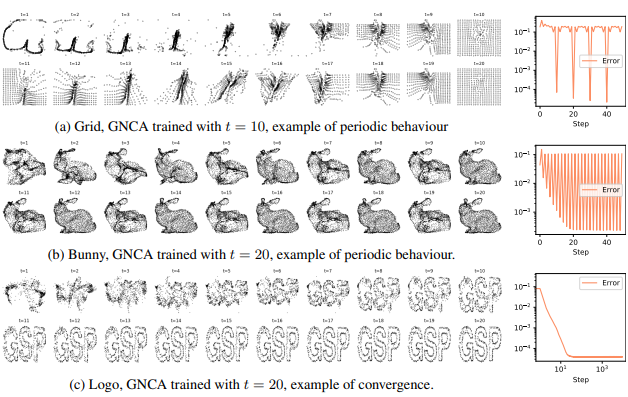
\includegraphics[width=\textwidth]{images/gnca-loss.png}
    \caption{State of each point cloud between $t=10$ and $t=20$ alongside mean squared error between current and target state \cite{grattarola2021learning}}
    \label{fig:gnca-loss}
\end{figure}

